\documentclass[tikz]{standalone}
\usepackage{fontspec}
\renewcommand*{\familydefault}{\sfdefault}
\usepackage{standalone}
\usepackage{amssymb}
\usetikzlibrary{decorations}
\usetikzlibrary{arrows.meta, decorations.pathmorphing, decorations.pathreplacing, shapes.geometric}
\usetikzlibrary{bayesnet}

\begin{document}

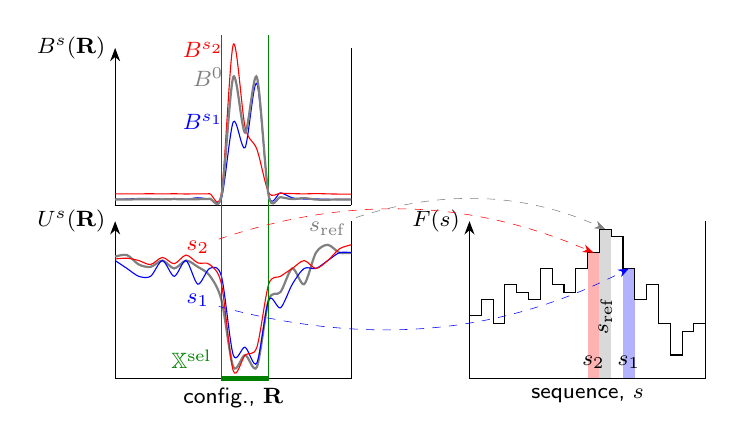
\begin{tikzpicture}[font=\footnotesize, xscale=1.5]

% axes
\draw[-Stealth] (-1,0) -- (-1,2) node[anchor=east] {\(U^s(\mathbf{R})\)} ;
\draw (1,0) -- (1,2) ;
\draw (-1,0) -- node[anchor=north] {config.,~\(\mathbf{R}\)} (1,0) ;

% selection subspace
\draw[ultra thick, green!50!black]
(-0.10,0) coordinate (X-sel-L) -- (+0.30,0) coordinate (X-sel-R)
;
\node[green!50!black, anchor=south east] at (X-sel-L) {\(\mathbb{X}^\mathrm{sel}\)};

% reference energy landscape s0
\draw[thick, gray] plot[smooth] coordinates {
(-1.0,1.55) (-0.9,1.57) (-0.8,1.45) (-0.7,1.42) (-0.6,1.50) (-0.5,1.40)
(-0.4,1.50)
(-0.3,1.42) (-0.2,1.31) (-0.1,1.0) (0.0,0.15) (0.1,0.3) (0.2,0.15) (0.3,1.0)
(0.4,1.1) (0.5,1.4) (0.6,1.2) (0.7,1.6) (0.8,1.7) (0.9,1.60) (1.0,1.6)
};

% energy landscape s1
\draw[blue] plot[smooth] coordinates {
(-1.0,1.5) (-0.9,1.4) (-0.8,1.3) (-0.7,1.3) (-0.6,1.5) (-0.5,1.3) (-0.4,1.5)
(-0.3,1.2) (-0.2,1.4) (-0.1,1.3) (0.0,0.3) (0.1,0.4) (0.2,0.2) (0.3,1.0) (0.4,0.9) (0.5,1.2) (0.6,1.4) (0.7,1.4) (0.8,1.5) (0.9,1.6) (1.0,1.6)
};

% energy landscape s2
\draw[thin, red] plot[smooth] coordinates {
(-1.0,1.52) (-0.9,1.53) (-0.8,1.5) (-0.7,1.45) (-0.6,1.54) (-0.5,1.46)
(-0.4,1.57)
(-0.3,1.47) (-0.2,1.45) (-0.1,1.2) (0.0,0.1) (0.1,0.3) (0.2,0.4) (0.3,1.2)
(0.4,1.3) (0.5,1.4) (0.6,1.5) (0.7,1.4) (0.8,1.5) (0.9,1.65) (1.0,1.7)
};

\begin{scope}[yshift=2.2 cm]

% axes
\draw[-Stealth] (-1,0) -- (-1,2) node[anchor=east] {\(B^s(\mathbf{R})\)} ;
\draw (1,0) -- (1,2) ;
\draw (-1,0) -- (1,0) ;

% Boltzmann distributions

\begin{scope}[yscale=0.7, yshift=0.1 cm]

% selection subspace
\coordinate (top) at (0,3);
\draw[green!50!black, very thin]
(X-sel-L) -- (X-sel-L|-top)
(X-sel-R) -- (X-sel-R|-top)
;


% U^s
\draw[blue] plot[smooth] coordinates {
(-1.0,0.012)
(-0.9,0.017)
(-0.8,0.026)
(-0.7,0.026)
(-0.6,0.012)
(-0.5,0.026)
(-0.4,0.012)
(-0.3,0.039)
(-0.2,0.017)
(-0.1,0.026)
(-0.0,1.415)
(+0.1,0.948)
(+0.2,2.11)
(+0.3,0.086)
(+0.4,0.128)
(+0.5,0.039)
(+0.6,0.017)
(+0.7,0.017)
(+0.8,0.012)
(+0.9,0.008)
(+1.0,0.008)
};

% U^s_2
\draw[thin, red, yshift=0.1 cm] plot[smooth] coordinates {
(-1.0,0.009)
(-0.9,0.009)
(-0.8,0.01)
(-0.7,0.012)
(-0.6,0.009)
(-0.5,0.012)
(-0.4,0.008)
(-0.3,0.011)
(-0.2,0.012)
(-0.1,0.033)
(-0.0,2.718)
(+0.1,1.221)
(+0.2,0.819)
(+0.3,0.033)
(+0.4,0.022)
(+0.5,0.015)
(+0.6,0.01)
(+0.7,0.015)
(+0.8,0.01)
(+0.9,0.006)
(+1.0,0.005)
};

% reference
\draw[thick, gray] plot[smooth] coordinates {
(-1.0,0.008)
(-0.9,0.008)
(-0.8,0.012)
(-0.7,0.014)
(-0.6,0.01)
(-0.5,0.015)
(-0.4,0.01)
(-0.3,0.014)
(-0.2,0.021)
(-0.1,0.074)
(-0.0,2.226)
(+0.1,1.221)
(+0.2,2.226)
(+0.3,0.074)
(+0.4,0.05)
(+0.5,0.015)
(+0.6,0.033)
(+0.7,0.007)
(+0.8,0.005)
(+0.9,0.007)
(+1.0,0.007)
};

% annotations
\path
(-0.0,1.415) coordinate (peak-s1)
(-0.0,2.718) coordinate (peak-s2)
(-0.0,2.226) coordinate (peak-ref)
;
\path[anchor=east, align=center, fill=white]
(peak-s1) node[blue] {\(B^{s_1}\)}
(peak-s2) node[red] {\(B^{s_2}\)}
(peak-ref) node[gray] {\(B^0\)}
;

\end{scope}

\end{scope}

% landscape labels
\node[anchor=north, blue] at (-0.3,1.2) (Us1) {\(s_1\)};
\node[anchor=south, red] at (-0.3,1.47) (Us2) {\(s_2\)};
\node[anchor=south, gray] at (0.8,1.7) (Usref) {\(s_\mathrm{ref}\)};

% fitness landscape
\begin{scope}[xshift=3 cm]

% color bars for F(s1) and F(s2)
\fill[blue!30!white] (0.3,0) rectangle (0.4,1.4) ;
\fill[red!30!white] (0,0) rectangle (0.1,1.6) ;
\fill[gray!30!white] (0.1,0) rectangle (0.2,1.9) ;

% labels for s1 and s2
\path
(0.35,0) node[anchor=south] {\(s_1\)}
(0.05,0) node[anchor=south] {\(s_2\)}
(0.15, 0.80) node[rotate=90, anchor=center] {\(s_\mathrm{ref}\)}
;

% axes
\draw[-Stealth] (-1,0) -- (-1,2) node[anchor=east] {\(F(s)\)} ;
\draw (1,0) -- (1,2) ;
\draw (-1,0) -- node[anchor=north] {sequence, \(s\)} (1,0) (1,0) ;

% fitness landscape
\draw[black] plot[const plot] coordinates {
(-1.0,0.8) (-0.9,1.0) (-0.8,0.7) (-0.7,1.2) (-0.6,1.1) (-0.5,1.0) (-0.4,1.4) (-0.3,1.2) (-0.2,1.1) (-0.1,1.4) (0.0,1.6) (0.1,1.9) (0.2,1.8) (0.3,1.4) (0.4,1.0) (0.5,1.2) (0.6,0.7) (0.7,0.3) (0.8,0.6) (0.9,0.7) (1.0,0.7)
};

% energy to fitness mappings
\begin{scope}[-Stealth, dashed, very thin]
\draw[blue] (Us1) to[bend right] (0.35,1.4) ;
\draw[red] (Us2) to[bend left] (0.05,1.6) ;
\draw[gray] (Usref) to[bend left] (0.15,1.9) ;

\end{scope}

\end{scope}
\end{tikzpicture}

\end{document}

